%%%%%%%%%%%%%%%%%%%%%%%%%%%%%%%%%%%%%%%%%
% Formal Book Title Page
% LaTeX Template
% Version 2.0 (23/7/17)
%
% This template was downloaded from:
% http://www.LaTeXTemplates.com
%
% Original author:
% Peter Wilson (herries.press@earthlink.net) with modifications by:
% Vel (vel@latextemplates.com)
%
% License:
% CC BY-NC-SA 3.0 (http://creativecommons.org/licenses/by-nc-sa/3.0/)
% 
% This template can be used in one of two ways:
%
% 1) Content can be added at the end of this file just before the \end{document}
% to use this title page as the starting point for your document.
%
% 2) Alternatively, if you already have a document which you wish to add this
% title page to, copy everything between the \begin{document} and
% \end{document} and paste it where you would like the title page in your
% document. You will then need to insert the packages and document 
% configurations into your document carefully making sure you are not loading
% the same package twice and that there are no clashes.
%
%%%%%%%%%%%%%%%%%%%%%%%%%%%%%%%%%%%%%%%%%

%----------------------------------------------------------------------------------------
%	PACKAGES AND OTHER DOCUMENT CONFIGURATIONS
%----------------------------------------------------------------------------------------

\documentclass[a4paper, 11pt, oneside]{book} % A4 paper size, default 11pt font size and oneside for equal margins

\usepackage[utf8]{inputenc} % Required for inputting international characters
\usepackage[T1]{fontenc} % Output font encoding for international characters
\usepackage{fouriernc} % Use the New Century Schoolbook font

\usepackage{listings}    % Include the listings-package
\lstset{language=C}   

\usepackage{xcolor}
\usepackage{float}


%\documentclass[letterpaper,12pt]{article}
\usepackage{tabularx} % extra features for tabular environment
\usepackage{amsmath}  % improve math presentation
\usepackage{graphicx} % takes care of graphic including machinery
\usepackage[margin=1in,letterpaper]{geometry} % decreases margins
\usepackage{cite} % takes care of citations
\usepackage[final]{hyperref} % adds hyper links inside the generated pdf file
\hypersetup{
	colorlinks=true,       % false: boxed links; true: colored links
	linkcolor=blue,        % color of internal links
	citecolor=blue,        % color of links to bibliography
	filecolor=magenta,     % color of file links
	urlcolor=blue         
}
\usepackage{blindtext}
%++++++++++++++++++++++++++++++++++++++++

%----------------------------------------------------------------------------------------
%	TITLE PAGE
%----------------------------------------------------------------------------------------

\begin{document} 

\begin{titlepage} % Suppresses headers and footers on the title page

	\centering % Centre everything on the title page
	
	\scshape % Use small caps for all text on the title page
	
	\vspace*{\baselineskip} % White space at the top of the page
	
	%------------------------------------------------
	%	Title
	%------------------------------------------------
	
	\rule{\textwidth}{1.6pt}\vspace*{-\baselineskip}\vspace*{2pt} % Thick horizontal rule
	\rule{\textwidth}{0.4pt} % Thin horizontal rule
	
	\vspace{0.75\baselineskip} % Whitespace above the title
	
	{\LARGE Run and Shoot} % Title
	
	\vspace{0.75\baselineskip} % Whitespace below the title
	
	\rule{\textwidth}{0.4pt}\vspace*{-\baselineskip}\vspace{3.2pt} % Thin horizontal rule
	\rule{\textwidth}{1.6pt} % Thick horizontal rule
	
	\vspace{2\baselineskip} % Whitespace after the title block
	
	%------------------------------------------------
	%	Subtitle
	%------------------------------------------------
	
	Software Design \& Project Set-up (Deliverable 2) % Subtitle or further description
	
	\vspace*{3\baselineskip} % Whitespace under the subtitle
	
	%------------------------------------------------
	%	Editor(s)
	%------------------------------------------------
	
	Students:
	
	\vspace{0.5\baselineskip} % Whitespace before the editors
	
	{\scshape\Large El-Habrouk Jaser \\ Firoozishahmirzadi Parichehreh \\ Layeghi Mahsa \\ Xu Jin} 
	
	\vspace{3\baselineskip} 
	
	%\textit{Carleton University} % Editor affiliation
	
		
	Course Instructor:
	
	\vspace{0.5\baselineskip} % Whitespace 
	
	{\scshape\Large Cristina Ruiz Martin}
	
	\vspace{3\baselineskip} % Whitespace 
	
	Course Title:
	\vspace{0.5\baselineskip} % Whitespace 
	
	{\scshape\Large Software Development with C} 
	
	\vfill % Whitespace between editor names and publisher logo
	
	%------------------------------------------------
	%	Publisher
	%------------------------------------------------
	
	
	\vspace{0.3\baselineskip} % Whitespace under the publisher logo
	
	Tuesday, 20\textsuperscript{th} of October, 2020 % Publication year
	

\end{titlepage}

%----------------------------------------------------------------------------------------



\section{Data Flow Diagram}

Data Flow Diagram or Flow chart explains the flow of our program since execution until finishes. 
\begin{figure}[ht] 
       
        \centering 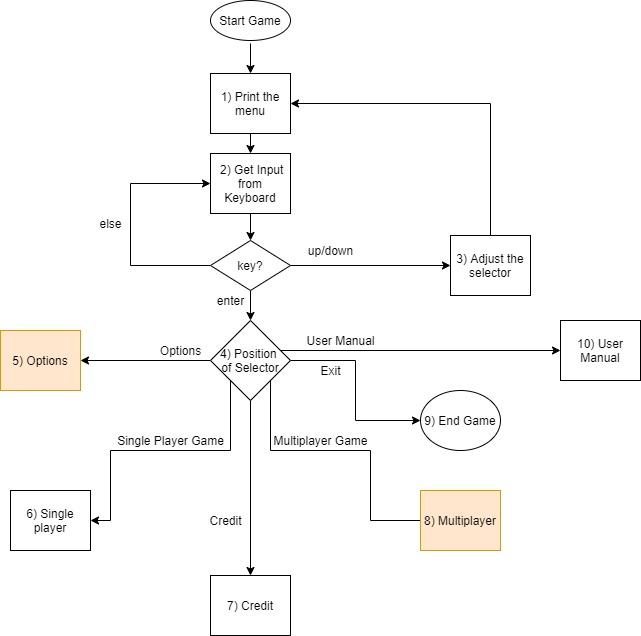
\includegraphics[width=0.8\columnwidth]{Run_and_shoot-Page-1}
        \caption{
        Flow Chart of Run and Shoot Game - Game Menu}
        \label{fig:menu}
\end{figure}

\subsection{Explanation of Flow Chart Figure 1}
NOTE:\emph{ The steps of the flow chart which are colored in  \textcolor{red}{ORANGE} indicates that they are going to be implemented for the second release.}

\vspace{0.5\baselineskip} % Whitespace 

As it is shown in Figure \ref{fig:menu}, initially, we print a menu for a player. There are multiple choices on the game menu and the player can go through each of them and hit enter to select one of them. So we are waiting for the player to enter \textbf{keys from input}.
We have a selector which places besides each option; The player can see the selector and be informed on its selection. This will done entirely on \textbf{Adjust the Selector} step of the flow chart.
In the next step we decide what to do next based on the player's choice. As we seen in Figure \ref{fig:menu}, we may go on six different steps resulting from \textbf{Position of Selector}. These are User Manual, Single Player Setup, Multiplayer Setup, options, credit and exit which will be explained in detail on another flowchart.






%\blindtext %delete this line

\begin{figure}
       
        \centering 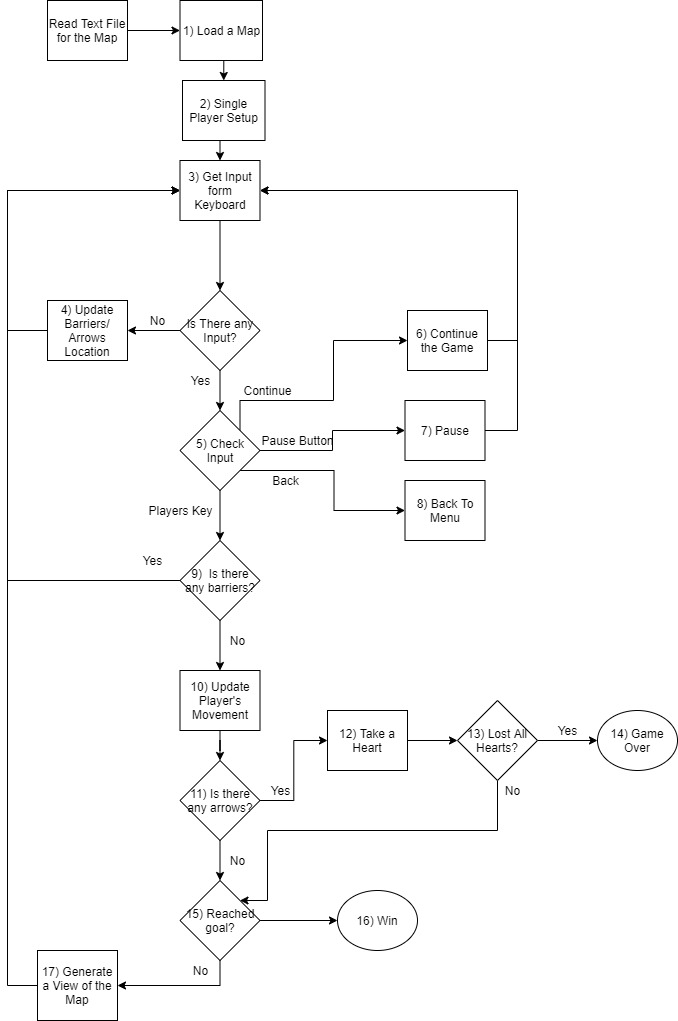
\includegraphics[width=0.9\columnwidth]{Run_and_shoot-Page-2}
        \caption{
        Flow Chart of Run and Shoot Game - Single Player}
        \label{fig:singleplayer}
\end{figure}

\subsection{Explanation of Flow Chart Figure 2}
This Flow chart explains all the steps happening on a \textbf{single player} mode. 
As it is shown in Figure \ref{fig:singleplayer}, on the \textbf{Load Map} step we should read the map from a text file. Next, We do some setups for single player game based on the map. In These setups we define a map with position of the player, the goal, the barriers and the arrows.
We should then \textbf{Get Input from Keyboard}. We should check if there was \textbf{any input from the player}. If not, we should \textbf{update the position of barriers/arrows} as they are moving objects. If the player hits pause button we go to the state of \textbf{pause game}. If hits on back button we \textbf{ get back to menu}. If hits continue we should \textbf{continue the game}.In both \textbf{continue} and \textbf{pause} state, we go back to \textbf{Get Input from Keyboard} and waits for the player to enter another key.

If the player push arrow keys or player's key we first check if the player's move is permitted or not; As there are statistic/moving barriers on the map, the player may not be allowed to go further on the map. Hence, we go to check \textbf{Is there any barriers?}. If there is one, we should go back to get input from keyboard step. If there wasn't any barriers on the way of the player, we go to the next step which is \textbf{Update Player's Movement}.

Next we check whether this movement made the player hit one of the arrows on the map. So we go to \textbf{Is there any Arrows?}. In this step if the player hits an arrow, we go to \textbf{Take a Heart} step to decrease one of the player's heart and immediately check if there is any hearts left or not on the \textbf{Lost All Hearts} state. If the player lost all of its hearts, we should end the game and go to \textbf{Game Over} step. Otherwise, we go to \textbf{Reach Goal state}; If the player has reached the goal, the player wins the game and we go to \textbf{Win} step. If the player has not reached the goal yet we first \textbf{Generate a view of the Map} to display any updates on the map causing by moving arrows/barriers and the player. Then we repeat all of these process from \textbf{Get Input from Keyboard} step until the player lose or win the game.

\begin{figure} 
       
        \centering 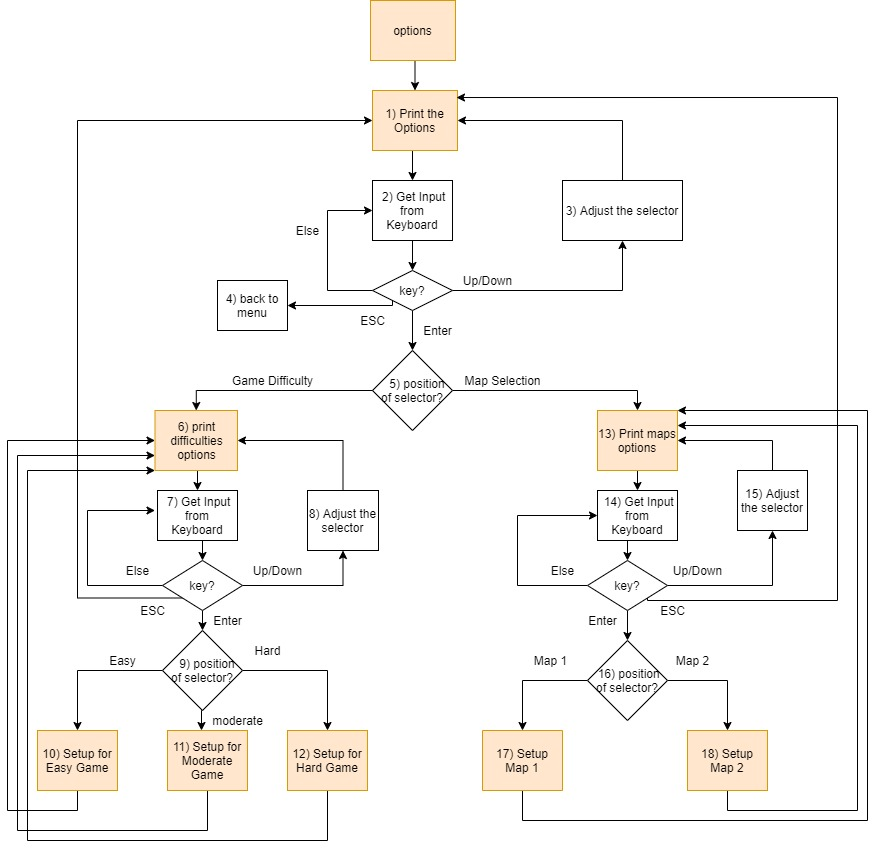
\includegraphics[width=\columnwidth]{Run_and_shoot-OPTIONS.jpg}
        \caption{
        Flow Chart of Run and Shoot Game - Options}
        \label{fig:options}
\end{figure}


\subsection{Explanation of Flow Chart Figure 3}
NOTE:\emph{ The steps of the flow chart which are colored in  \textcolor{red}{ORANGE} indicates that they are going to be implemented for the second release. As some of these steps are repeated in single player mode, we didn't colored them in Orange}

\vspace{0.5\baselineskip} % Whitespace 

This Flow chart explains all the steps happening on a \textbf{Options} mode. 
As it is shown in Figure \ref{fig:options} initially,on the \textbf{Print the Options} we print the options for the player. We \textbf{Get input from keyboards}.
We have a selector which places besides each option; The player can see the selector and be informed on its selection. If the player hits up or down keys, we \textbf{Adjust the Selector}. If hits on ESC button we \textbf{Back to Menu}. If hits enter we go to the next step which is \textbf{Position of Selector}.

At this step, We \textbf{Print Difficulties Options} and \textbf{Maps Options} according to player's choice.

In each of \textbf{Print Difficulties Options} and \textbf{maps options}, we \textbf{Get input from keyboards} again and all the \textbf{Adjust the Selector} and pressing ESC button process will happen again.

If the player hits enter on \textbf{Game difficulty} flow, we go to \textbf{Position of Selector} step. Once the player chooses a level out of three levels, the game will be setup for the level chosen \textbf{Setup for Easy/moderate/hard Game} and we will then go back to \textbf{Print Difficulties Options}. if the players presses on ESC then we will go back to the \textbf{Print the options}.

If the player hits enter on \textbf{Map selection} flow, we go to \textbf{Position of Selector} step. Once the player chooses a Map from two maps, we setup the game to use the selected Map \textbf{Setup map 1 or Setup map 2} and we go back to \textbf{Map selection}.  If the players hits ESC we go back to \textbf{Print the Options}.

\begin{figure} 
       
        \centering 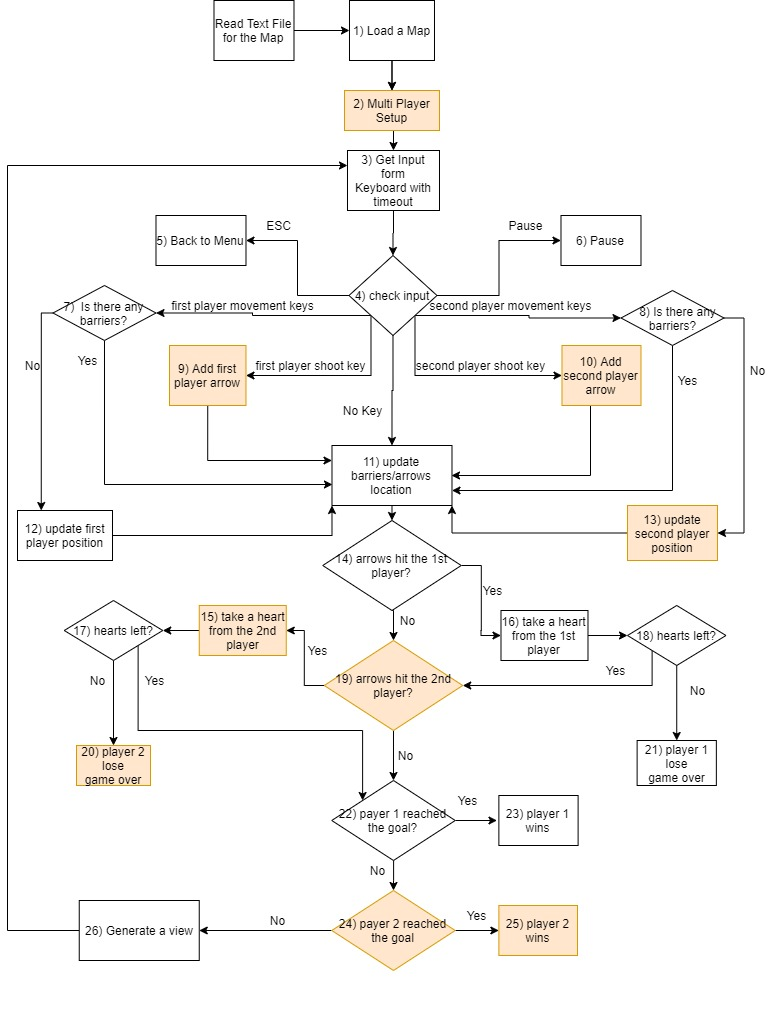
\includegraphics[width=\columnwidth]{Run_and_shoot-MULTI_PLAYER.jpg}
        \caption{
        Flow Chart of Run and Shoot Game - Multi Player}
        \label{fig:multiplayer}
\end{figure}


\subsection{Explanation of Flow Chart Figure 4}





\newpage
\section{Functions}
\subsection{Definition}
The following is just struct type declaration and some definitions for our game and it is needed for function's parameters or return type of functions.

\vspace{0.5\baselineskip} % Whitespace 

\begin{lstlisting}[frame=single]  % Start your code-block

#define MAX_ITEM_SIZE 100
#define NUM_OF_ITEMS 5
#define MAP_MAX_NUM_OF_BARRIERS 10
#define MAP_MAX_NUM_OF_ARROWS 20

typedef struct MenuItem {
	char str[MAX_ITEM_SIZE];
} MenuItem;

typedef struct Menu {
	int selector;
	MenuItem items[NUM_OF_ITEMS];
} Menu;


typedef struct OptionItem {
	char str[MAX_ITEM_SIZE];
} OptionItem;

typedef struct option {
	int selector;
	OptionItem items[NUM_OF_ITEMS];
} Option;

typedef struct Position {
	int x;
	int y;
} Position;

typedef enum {
	DIRECTION_RIGHT,
	DIRECTION_LEFT,
	DIRECTION_UP,
	DIRECTION_DOWN
} Direction;

typedef enum {
	SPEED_LOW,
	SPEED_NORMAL,
	SPEED_HIGH,
} Speed;

typedef struct MapSpace {
	int xMin;
	int xMax;
	int yMin;
	int yMax;
} MapSpace;

typedef struct MapBarrier {
	Position currentPos;
	int length;
	Direction currectDir;
} MapBarrier;

typedef struct MapArrow {
	Position currentPos;
	Speed speed;
} MapArrow;

typedef struct Player {
	Position currentPos;
	int heart;
} Player;

typedef struct Goal {
	Position goal;
} Goal;

typedef struct Map {
	MapSpace space;
	int numberOfBarriers;
	int numberOfArrows;
	MapBarrier barrier[MAP_MAX_NUM_OF_BARRIERS];
	MapArrow arrow[MAP_MAX_NUM_OF_ARROWS];
	Goal goal;
	Player player;
} Map;

\end{lstlisting}

\subsection{Functions Prototypes}
\subsubsection{Flow Chart - Game Menu}

\begin{lstlisting}[frame=single]

/* STEP 1
 * Prints the game start up menu on the consol.
 * Input: menu
 * Return: void */
void printMenu(Menu menu);

/* STEP 2
 * This is done entirely on the MAIN
*/

/* STEP 3
 * Updates the selector position according to input key.
 * Input: menu_p, arrowKey
 * Output: menu_p
 * Return: void*/
int updateMenuSelector(Menu* menu_p, int arrowKey);

/* STEP 4
 * This will call functions related to each option
 * Input: selector
 * Output: 
 * Return: void*/
void chooseMenuOption(int selector);

/* STEP 5
 * This will call functions related to OptionsMenu
 * Input: void
 * Output: void
 * Return: void*/
void OptionMenu(void);

/* STEP 6
 * This will call functions related to Single Player Setup 
 * on Level 2 flowchart
 * Input: void 
 * Output: void
 * Return: void */
void singlePlayer(void);

/* STEP 7
 * shows information about the credits
 * Input: void 
 * Output: void
 * Return: void */
void credit(void);

/* STEP 8
 * This will call functions related to Multiplayer Setup on -
 * Input: void 
 * Output: void
 * Return: void */
void multiPlayer(void);

/* STEP 9
 * Exit from the game
 * Input: void 
 * Output: void
 * Return: void */
void exit(void);

/* STEP 10
 * displays a user manual for the player; (How to Play)
 * Input: void 
 * Output: void
 * Return: void */
void userManual(void);

\end{lstlisting}



\subsubsection{Flow Chart - Single Player}
\begin{lstlisting}[frame=single]


/* STEP 1 and STEP 2
 * Load map information from an input file using provided information
 * from options.
 * Input: file_p, mapNumber
 * Output: Map */
Map loadMap(FILE* file_p,int mapNumber);

/* STEP 3
 * This is done entirely on the MAIN
*/

/* STEP 4
 * Update barrier position in the map
 * Input: barrier, space
 * Output: barrier */
void updateBarrier(MapBarrier* barrier, MapSpace space);

/* STEP 4
 * Update arrow position in the map
 * Input: arrow, space
 * Output: arrow
 * Return: void */
void updateArrow(MapArrow* arrow, MapSpace space);

/* STEP 5
 * This is done entirely on the MAIN
*/

/* STEP 6
 * It continues the game when the game is on pause 
 * Input: void
 * Return: void */
void continueGame(void);

/* STEP 7
 * It pause the game
 * Input: void
 * Return: void */
void pauseGame(void);

/* STEP 8
 * It goes back to Menu
 * Input: void
 * Return: void */
void backToMenu(void);


/* STEP 9
 * Check if there is any barrier on the way of player.
 * Input: player, barrier
 * Output: 0 ---> player is hit & 1---> player not hit
 * Return: int */
int isBarrier(Player player,MapBarrier* barrier);

/* STEP 10
 * Update player position in the map.
 * Input: player, arrowKey
 * Output: player 
 * Return: void*/
void updatePlayerPos(Player *player, int arrowKey);

/* STEP 11
 * check if the player is hit by arrows.
 * Input: player, arrow
 * Output: 1 ---> if the player is hit
 * Return: int */
int isPlayerHit(Player player, MapArrow* arrow );


/* STEP 12
 * Takes a heart from the player.
 * Input: player
 * Output: player
 * Return: void */
void lostHeart(Player player);

/* STEP 13
 * Check if the player lost all its heart.
 * Input: player
 * Output: 1 ---> if the player lost all its heart
 * Retun: int */
int isGameOver(Player player);

/* STEP 14
 * inform player that he/she lost the game
 * Input: player
 * Output: void
 * Return: void*/
void gameOver(Player player);


/* STEP 15
 * Cheak if the player reach the goal
 * Input: player, goal
 * Output: 1 ---> if the player reach the goal
 * Return: int */
int reachGoal(Player player, Goal goal);

/* STEP 16
 * inform player that he/she win the game
 * Input: player
 * Output: void
 * Return: void*/
void winGame(Player player);

/* STEP 17
 * Generate a map using updated information
 * Input: map
 * Return: void */
void updateView(Map map);


\end{lstlisting}

\subsection{Flow Chart - Options}
\begin{lstlisting}[frame=single]

/* STEP 1 and STEP 6 and STEP 13
 * Prints the options on the consol.
 * Input: option
 * Return: void */
void printOption(Option option);

/* STEP 2 and STEP 7 and STEP 14
 * This is done entirely on the MAIN
*/

/* STEP 3 and STEP 8 and STEP 15
 * Updates the selector position according to input key.
 * Input: option_p, arrowKey
 * Output: option
 * Return: void*/
void updateOptionSelector(Option* option_p, int arrowkey);

/* STEP 4
 * It goes back to Menu
 * Input: void
 * Return: void */
void backToMenu(void);

/* STEP 5 and STEP 9 and STEP 16
 * This will call functions related to each option
 * Input: selector
 * Output: 
 * Return: void*/
void chooseMenuOption(int selector);


/* STEP 10 and STEP 11 and STEP 12
 * select a difficulty level
 * Input: option, key
 * Output: difficulty level
 * Return: int */
void setDifficulty(Option option, int key);

/* STEP 17 and STEP 18
 * select a map
 * Input: option, key
 * Output: map number
 * Return: int */
int setMap(Option option, int key);

\end{lstlisting}

\subsection{Flow Chart - MultiPlayer}
\begin{lstlisting}[frame=single]

/* STEP 1 and STEP 2
 * Load map information from an input file using provided information
 * from options.
 * Input: file_p, mapNumber
 * Output: Map */
Map loadMap(FILE* file_p,int mapNumber);

/* STEP 3 and STEP 4
 * This is done entirely on the MAIN
*/

/* STEP 5
 * It goes back to Menu
 * Input: void
 * Return: void */
void backToMenu(void);

/* STEP 6
 * It pause the game
 * Input: void
 * Return: void */
void pauseGame(void);


/* STEP 7 and STEP 8
 * Check if there is any barrier on the way of player.
 * Input: player, barrier
 * Output: 0 ---> player is hit & 1---> player not hit
 * Return: int */
int isBarrier(Player player,MapBarrier* barrier);


/* STEP 9 and STEP 10
 * Generates and shoot an arrow
 * Input: player
 * Output: generated arrow
 * Return: Arrow */
Arrow shoot(Player player);

/* STEP 11
 * Update arrow position in the map
 * Input: arrow, space
 * Output: arrow
 * Return: void */
void updateArrow(MapArrow* arrow, MapSpace space);

/* STEP 11
 * Update barrier position in the map
 * Input: barrier, space
 * Output: barrier */
void updateBarrier(MapBarrier* barrier, MapSpace space);

/* STEP 12 and STEP 13
 * Update player position in the map.
 * Input: player, arrowKey
 * Output: player 
 * Return: void*/
void updatePlayerPos(Player *player, int arrowKey);

/* STEP 14 and STEP 19
 * check if the player is hit by arrows.
 * Input: player, arrow
 * Output: 1 ---> if the player is hit
 * Return: int */
int isPlayerHit(Player player, MapArrow* arrow );

/* STEP 15 and STEP 16
 * Takes a heart from the player.
 * Input: player
 * Output: player
 * Return: void */
void lostHeart(Player player);


/* STEP 17 and STEP 18
 * Check if the player lost all its heart.
 * Input: player
 * Output: 1 ---> if the player lost all its heart
 * Retun: int */
int isGameOver(Player player);


/* STEP 20 and STEP 21
 * inform player that he/she lost the game
 * Input: player
 * Output: void
 * Return: void*/
void gameOver(Player player);

/* STEP 22 and STEP 24
 * Cheak if the player reach the goal
 * Input: player, goal
 * Output: 1 ---> if the player reach the goal
 * Return: int */
int reachGoal(Player player, Goal goal);

/* STEP 23 and STEP 25
 * inform player that he/she win the game
 * Input: player
 * Output: void
 * Return: void*/
void winGame(Player player);

/* STEP 26
 * Generate a map using updated information
 * Input: map
 * Return: void */
void updateView(Map map);


\end{lstlisting}

\end{document}
